
\section{Tectonic seismic zones and seismicity parameters}
\noindent
Iran is situated over Himalayan-Alpide seismic belt, which has frequently experienced strong shaking induced by earthquakes. These earthquakes are categorized in various tectonic seismic zones. Based on seismicity parameters different tectonic seismic devisions have been defined for Iran.  Some studies defined more detailed division \citep{Nowroozi1976, Tavakoli1999}, and some of them defined one simplified province \citep{Stocklin1968, Takin1972, Berberian1976}. \citet{Mirzaei1998} divided Iran into five tectonic regions, including Azerbaijan-Alborz, Kopeh-Dagh, Zagros, Central-East Iran, and Makran. Considering \citet{Mirzaei1998} devision, \citet{Karimiparidari2013} divided the Azerbaijan-Alborz tectonic seismic region into two regions, which are Azerbaijan and Alborz Mountain Range (hereinafter, Alborz). Azerbaijan, Alborz and Kopeh-Dagh tectonic seismic regions encompass most of northern Iran.  Fig.~\ref{fig:study_region} shows the study region and tectonic seismic regions. \\

\begin{figure} [ht]
\centering
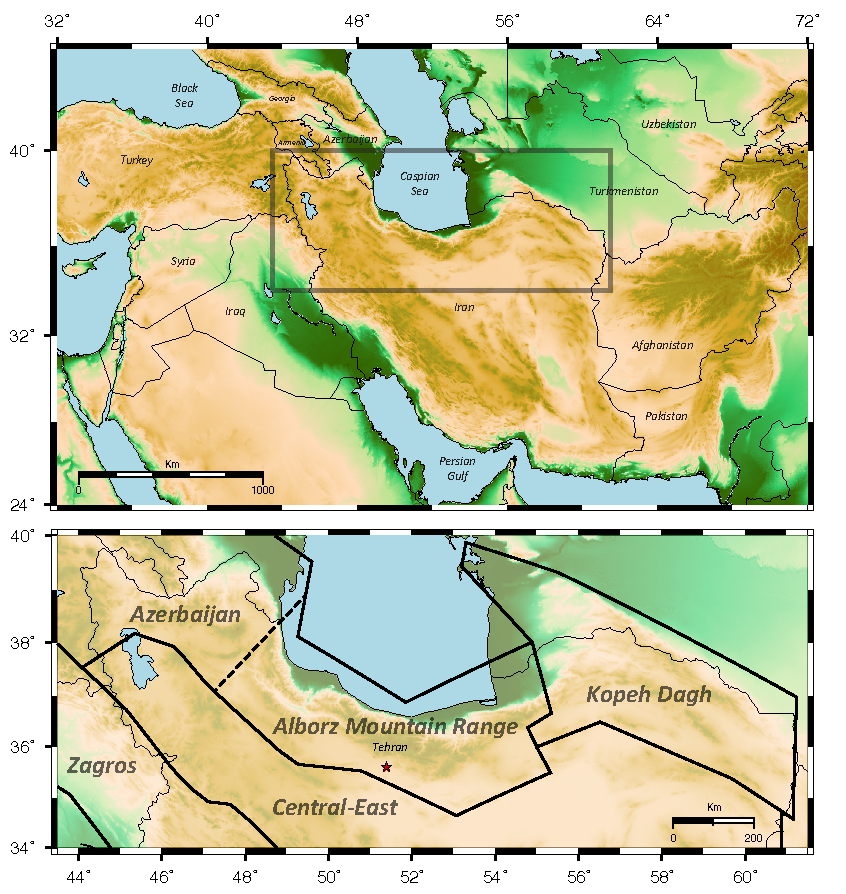
\includegraphics[scale=0.6]{figures/pdf/Figure01.pdf} 
\caption{a) Map of Iran and surrounding countries. The study area is presented in gray box. b) The study area containing seismotectonic provinces after \citet{Mirzaei1998}, and location of big cities. Dashed line is the subdivision that is proposed by \citet{Karimiparidari2013}}
\label{fig:study_region}
\end{figure}




\noindent
Alborz tectonic seismic region has active reverse faults, which are parallel to the northwest-trending structural gain of the Alborz Mountains belt. Here a series of historical earthquakes occurred within a time period of more than 1100 years. At least three damaging earthquakes in 958 (western segments), 1655 (eastern segments), and 1830 (central segments), ruptured adjacent segments of the Mosha fault, located in northern Tehran.  The North Tehran Thrust (NTT) adds more complexity due to the presence of south-dipping reverse faults, which are in part blind, such as the Davudieh, Shian, and Bagh-E Feyz.
The northwest continuation of the Alborz Mountains, known as the Rocks of the Talesh Mountains, have been thrust northeastward and eastward over rocks of the south Caspian depression. An earthquake with Ms 6.0 in 1978 led to a focal mechanism consistent with a low-angle thrust \citep{Berberian1999}. 

\noindent
There were three earthquakes from 1721-86 that ruptured the North Tabriz Fault system from southeast to northwest, as part of Azerbaijna tectonic seismic zone. The Tabriz region is in the Araxes structural block of northwestern Iran, southwest of the continuation of the western Alborz Mountains towards the Caucasus. The North Tabriz Fault (NTF) is a complex northwest-trending structure, which contains evidence observed on aerial photographs, and vertical displacement with the north side up, of right-lateral strike-slip displacement \citep{Berberian1999}.

The NTF system and nearby reverse faults ruptured from southeast to northwest in three earthquakes over 65 years: the Shebli earthquake with magnitude 7.3 in 1721 on the southeastern NTF with a surface rupture more than 35 km long, reported by \citet{Jones1834} the Tabriz earthquake with magnitude 7.4 in 1780 on the northwestern NTF, with a surface rupture more than 42 km long and vertical separation of 2 to 4 m; and the Marand-Mishu earthquake with magnitude of 6.3 in 1786 on the Mishu reverse fault and the Sufian segment of the NTF. Another earthquake with  magnitude 5.5 struck the Tasuj reverse fault farther west in 1807 and an earthquake of M 6.7 took place along the South Bozqush reverse fault farther southeast in 1879. Prior to the 1721-86 earthquake sequence, Tabriz was shaken by earthquakes in 858 (M 6.0), 1042 (M 7.3), 1273 (M ~ 6.5), and 1304 (M 6.7)\citep{Berberian1999}. Most recently, earthquakes with Mw 6.1 in 1997 and Mw 6.4 in 2012 occurred in Ardabil and Tabriz, respectively. 


The main Kopeh-Dagh fault system has experienced some historic earthquakes. Ashgabat, the capital city of Turkmenistan, was destroyed by an earthquake of $Ms$ 7.2 in 1948 and destroyed more than 30 villages in Iran. This was the strongest earthquake to strike this region since at least 1455.
The main Kopeh-Dagh fault consists of several partly overlapping segments parallel to the overall $NW - SE$ structure with step-overs. The regions of overlap are characterized by shorter south-dipping thrust faults striking about E - W \citep{Berberian2001}. \citet{Trifonov1978} reported active displacement along the main Kopeh-Dagh fault for more than 500 km. 
Massive destruction of the capital city of Mithradatkert is attributed to the 10 BC event Ms 7.1, roughly 30 kilometers from the border of Iran (Nesa mound) \citep{Berberian2001}.
The Neyshabur sequence of four earthquakes between 1209 and 1405 respected the segment boundary between the Neyshabur and Binalud reverse fault system \citep{Berberian1999}.
Historical records show that in 1209, the district of Neyshabur from Neyshabur city in the west to Daneh village in the east was totally destroyed \citep{Berberian1999}.

\subsection{Magnitude Conversion}
\noindent
The catalog of recorded earthquake from 2005-2015 which is downloaded from IIEES is reported the earthquake based on different magnitude scale (reference). We converted the $M_L$, $M_S$, and $mb$ magnitudes through conversion relationships which is defined in \citet{Zare2014}. There also some of data which is recorded in $M_D$ (Duration magnitude). These data are reported by International Seismological Centre (ISC).  \citet{Deniz2010} developed a set of empirical equations to convert earthquake magnitudes in $mb$, $M_D$, $M_L$ and $M_S$ scales to the $M_W$ scales using orthogonal regression procedure. They used data of earthquake that occurred in Turkey from different data centers including ISC. In this study we use the conversion equation of \citet{Deniz2010} to convert the $M_D$ to $M_W$. Although they defined the equation based on $4.5\leqslant M_W$, we extrapolate the equation for lower magnitude. We believe having those earthquakes, even with small error  in magnitude is important for estimating an accurate  Gutenberge-Richter values.

\subsection{Declustering}
\noindent
It is generally assumed that the seismicity of each tectonic seismic source follows a Poissonian occurrence process. Therefore, in order to accomplish this, we declustered the earthquake catalog. In compiling the catalog of events, foreshocks and aftershocks were removed using a declustering methodology \citet{Gardner1974}. Fig.~\ref{fig:seismicity} shows the epicenter of declustered instrumental  earthquakes.

\begin{figure} [ht]
\centering
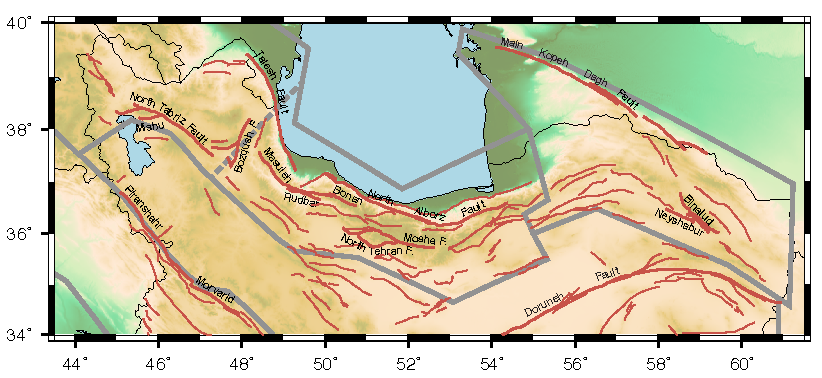
\includegraphics[scale=0.6]{figures/pdf/Figure02.pdf} 
\caption{Declustered instrumental seismicity map (2005 - 2015) of Northern Iran.}
\label{fig:seismicity}
\end{figure}


\subsection{Catalog Completeness}
\noindent
Completeness of catalog is an important factor in studying the earthquake sequence.  In this study we used the Maximum curvature method (MAXC) \citep{Wiemer2000}. According to MAXC method, a complete catalog should follow the Gutenberg-Richter power law distribution of magnitude. The steps for picking the completeness magnitude for each catalog include, 1) Calculating the $a-$ and $b-$ value based on the minimum magnitude, 2) generate  synthetic events based on the achieved value that the cumulative number of events obey the power law distribution, 3) Calculate the goodness of fit for predicted and observed cumulative numbers for each magnitude bin. Higher \citep{Wiemer2000}. We increase the minimum magnitude and repeat the process. For each tectonic seismic region, we pick the magnitude corresponding to the highest goodness of fit.  \citet{Wiemer2000} assumed the threshold of goodness of fit as 90\% in order to completeness of the catalog, however,  not all frequency-magnitude distributions reach the 90\% mark. Fig.~\ref{fig:completeness} , shows the goodness of fit value for three tectonic seismic regions. 

\begin{figure} [ht]
\centering
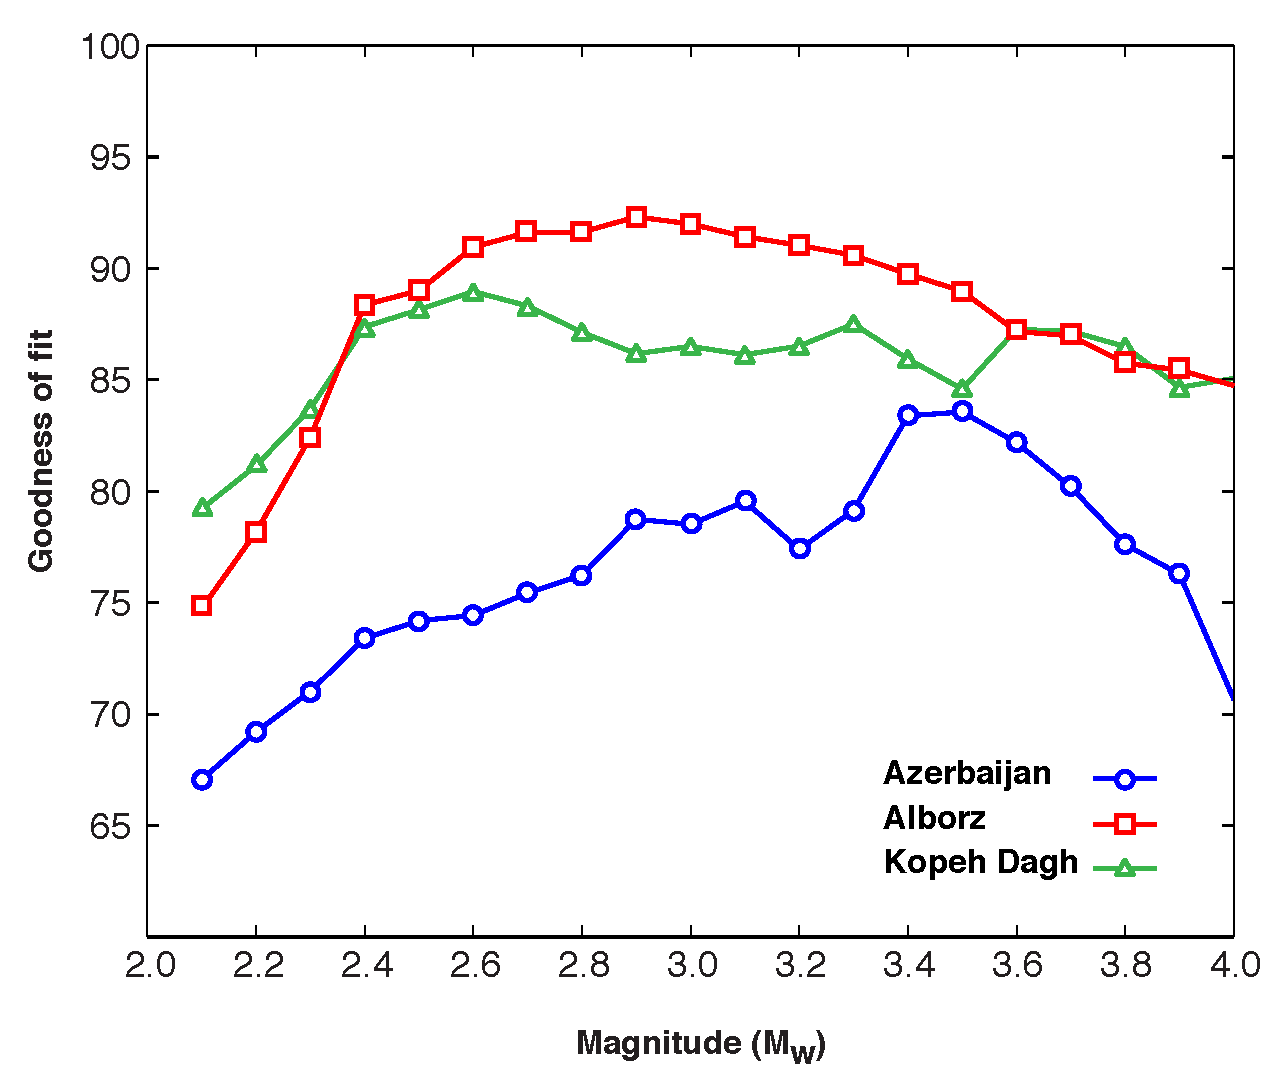
\includegraphics[scale=0.4]{figures/pdf/Figure03.pdf} 
\caption{Goodness of fit value of MAXC method for three tectonic seismic regions for seismicity of 2005-2015 (a) Azerbaijan b)Alborz c) Kopeh Dagh)}
\label{fig:completeness}
\end{figure} 





\noindent
In this study we assumed the minimum magnitude for complete recording, $M_C$, are 2.9, 3.5, and 2.6 for Alborz, Azerbaijan, and Kopeh Dagh, respectively. Fig.~\ref{fig:mag-time} shows the magnitude time series of the declustered data for three regions. Earthquake with magnitude bigger than completeness magnitude are represented. 

\begin{figure} [ht]
\centering
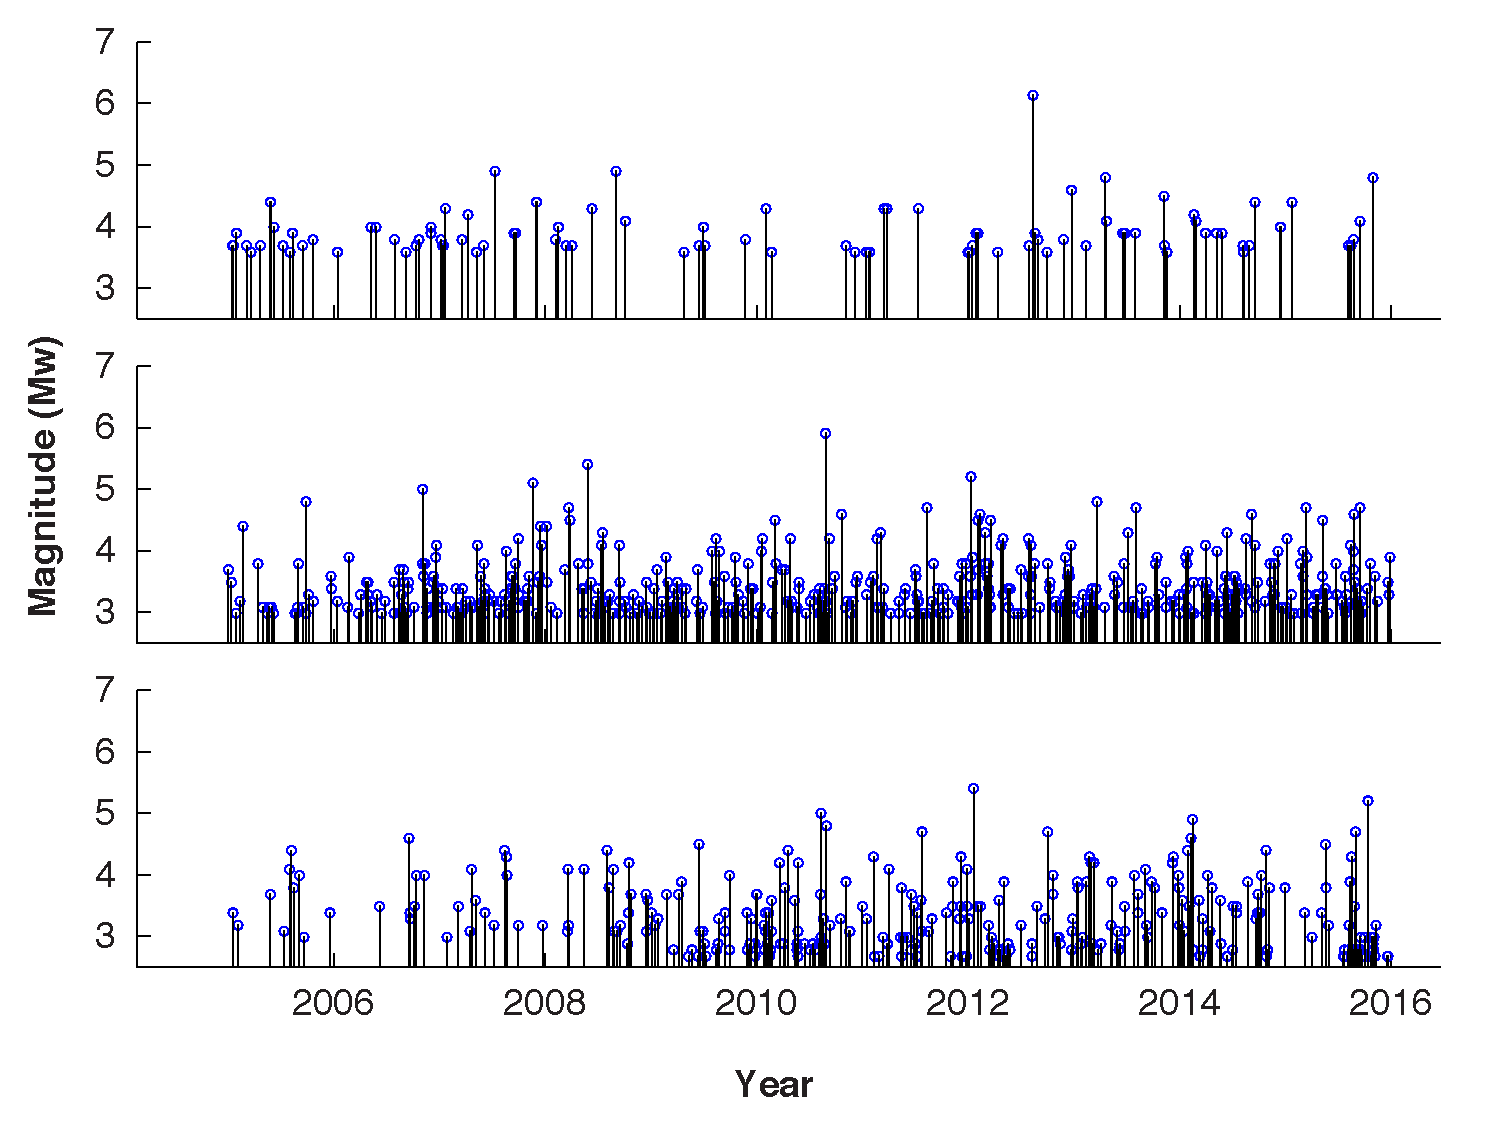
\includegraphics[scale=0.5]{figures/pdf/Figure04.pdf} 
\caption{Variation of moment magnitude of earthquake in 2005-2015 for north Iran. (a) Azerbaijan b)Alborz c) Kopeh Dagh)}
\label{fig:mag-time}
\end{figure} 








